\documentclass[12pt, a4paper]{article}
\usepackage[utf8]{inputenc}

\title{Update of the register size used in the NeXtRad Synchronization Controller}
\author{Dominic Manthoko}
\date{\today}

%package needed in order to use images
\usepackage{graphicx}
\graphicspath{{images/}{images/tcu/}{images/tcu_external_clock}}

%hyperlinks
\usepackage{hyperref}
\hypersetup{
    colorlinks=true,
    linkcolor=blue,
    filecolor=magenta,      
    urlcolor=cyan,
}

\urlstyle{same}

\begin{document}

%\begin{titlepage}
\maketitle
%\end{titlepage}

%Deals with the text being too long to fill one line
%E.g Background of the NeXtRad...
\sloppy


\section{Introduction}

\subsection{Subject and Motivation of Report}
The author was requested to make modifications to the NeXtRad Synchronization Controller developed by Johann Burger. In particular, the register size of the Synchronization Controller needed to be increased from 16 bits to 32 bits. 

\subsection{Background of the NeXtRad Synchronization Controller}


\subsection{Methodology}

\section{The Synchronization Controller}
\subsection{Modifications Made to the Original Synchronization Controller}
It is highly recommended that you read the document about the \href{https://docs.google.com/document/d/1E-mxDRlNcjSsjckUj8SuQOPBRs8Zv4AUUxXzLDHU3zc/edit?usp=sharing}{Timing Control Unit(TCU)}. This document specifies how to set up the synchronization controller, the commands used to operate it and so forth. In this section, only the parts that were modified will be mentioned.

\begin{flushleft}

\end{flushleft}

\subsection{Setting up the Synchronization Controller}
All the available registers can be accessed in the proc directory:

	\begin{flushleft}
		\fbox{\begin{minipage}{30em}
		/proc/$<$PID$>$/hw/ioreg/
		\end{minipage}}
	\end{flushleft}

\begin{flushleft}
where $<$PID$>$ must be replaced by the process ID of the running firmware. This can be identified by running the ‘ps’ command in the terminal.
\end{flushleft}

\begin{flushleft}
Registers can be written to by using the echo command. The following command writes a 1 to the n register:

	%display an example of the echo command inside a box
	\begin{flushleft}
		\fbox{\begin{minipage}{30em}
			echo -e -n "\textbackslash x01\textbackslash x00" $>$ /proc/$<$PID$>$/hw/ioreg/n
		\end{minipage}}
	\end{flushleft}

\end{flushleft}

\begin{flushleft}
The registers can then be read back by using the ‘od’ command:

	%display an example of the od command inside a box
	\begin{flushleft}
		\fbox{\begin{minipage}{30em}
			od -x /proc/$<$PID$>$/hw/ioreg/n
		\end{minipage}}
	\end{flushleft}

\end{flushleft}

%Explaining how to use the TCU with the modifications
\begin{flushleft}
With the modified TCU, reading and writing from the n, m and reg\textunderscore led registers found in the proc directory was left unchanged. The reg\textunderscore pulse register was altered such that it would be able to handle 32 bit values for the PRI offset.
\end{flushleft}

%table describing the parameters used in the reg_pulses register
\begin{table}
\centering
\begin{tabular}{ |c|c|c|c| } 
 \hline
 Parameter & Size &  Description \\ 
 
 \hline 
 MB offset & 16 bits & Main Bang offset in 10ns intervals \\ 
 
 \hline
 DIG offset & 16 bits & Digitisation offset in 10ns intervals \\
 
 \hline
 Next PRI (upper 2 bytes) & 16 bits & Next PRI offset in 10ns intervals \\
 
 \hline
 Freq & 16 bits & Frequency of operation \\
 
 \hline
 Pol Mode & 3 btis & From table 1.2 \\
 
 \hline
 Next PRI (lower 2 bytes) & 16 bits & Next PRI offset in 10ns intervals\\
 \hline 
\end{tabular}
\caption{Table of all the parameters necessary for each pulse}
\label{table:1}
\end{table}

	\begin{figure}
		\centering
		\includegraphics[width=13cm]{reg_pulses}
		\caption{Visual depiction of how the parameters are setup using the echo command}
		\label{fig:reg_pulses}
	\end{figure}


\begin{flushleft}
The original developer catered for the future improvement of the controller and had 16 bits of unused bits available for use. This free space was made use of in order to increase the register size of the PRI from 16- to 32-bits. In table \ref{table:1}, the various parameters required to set up a pulse are shown. Figure \ref{fig:reg_pulses} shows how the parameters seen in table \ref{table:1} would be setup using the echo command.
\end{flushleft}

\begin{flushleft}
The parameters seen in table \ref{table:1} are set up by writing to the reg\textunderscore pulses register. If you wanted to set up a pulse that triggers every 1 ms (1Khz), has a main bang and digitisation offset of 500ns, a band frequency of 1300 MHz and operating at L-band, you would write the following command. 


	%display an example of the od command inside a box
	\begin{flushleft}
		\fbox{\begin{minipage}{30em}
			echo -e -n "\textbackslash x32\textbackslash x00\textbackslash x32\textbackslash x00\textbackslash x01\textbackslash x00\textbackslash x14\textbackslash x05\textbackslash x01\textbackslash x00\textbackslash x3b\textbackslash x86" $>$ /proc/$<$PID$>$/hw/ioreg/reg\textunderscore pulses
		\end{minipage}}
	\end{flushleft}
	
\end{flushleft}

%how to get the hex values for the main bang offset and the digitization offset
\begin{flushleft}
The Rhino operates using a 100MHz clock, which is 10ns cycles. For the main bang and digitization offset, we divide the desired offset by 10ns to get the number of cycles. Since we want an offset of 500ns for both of them, the number of cycles is equal to 50 (x0032 in hexadecimal). The value must be in little endian thus we set these to \textbackslash x32\textbackslash x00. 
\end{flushleft}

%how to get the hex values for the PRI offset
The desired PRI is calculated using the following equation:

	\[ 
		PRI = \frac{\frac{1}{PRF}}{10ns} - MB - D
	\]
Where
 
	\begin{itemize}
  		\item PRF is the frequency we want at the output i.e coming out of the main bang pin on the Rhino board
  		\item MB is the main bang offset in cycles
  		\item D is the digitization offset in cycles
	\end{itemize}

Since MB = D = 50 and we want a PRF of 1kHz, we get a value of 99899 for the PRI. Converting the value to hexadecimal we get x0001 863B. Then you would write \textbackslash x01\textbackslash x00 to PRI upper two bytes and \textbackslash x3b\textbackslash x86 to PRI lower two bytes.


\section{Experimental setup}

	\begin{figure}[h]
		\centering
		\includegraphics[width=13cm]{experimental_setup}
		\caption{Picture of the equipment used to test the 32 bit version of the synchronization controller}
		\label{fig:exp_setup}
	\end{figure}
	
The experimental setup used to test the modified controller can be seen in figure \ref{fig:exp_setup}. A signal generator operating at 100MHz with an amplitude of +550mV was used as the input clock. This clock signal was passed through a diode then fed into the rhino. An oscilloscope was used to measure the Main bang offset and Digitisation signals coming out of the rhino. 

\begin{flushleft}
Mention stuff about Xilinx IDe, computer specs, operating system and cabling used
\end{flushleft}
	
	
\section{Results of the Experiment}

\subsection{Using the Rhino Board Internal 100MHz clock}

Testing of the modified synchronization controller began with using the internal clock of the Rhino board. Using the internal clock, 1kHz, 2kHz, 3kHz and 4kHz signals were produced. 

	\begin{figure}
		\centering
		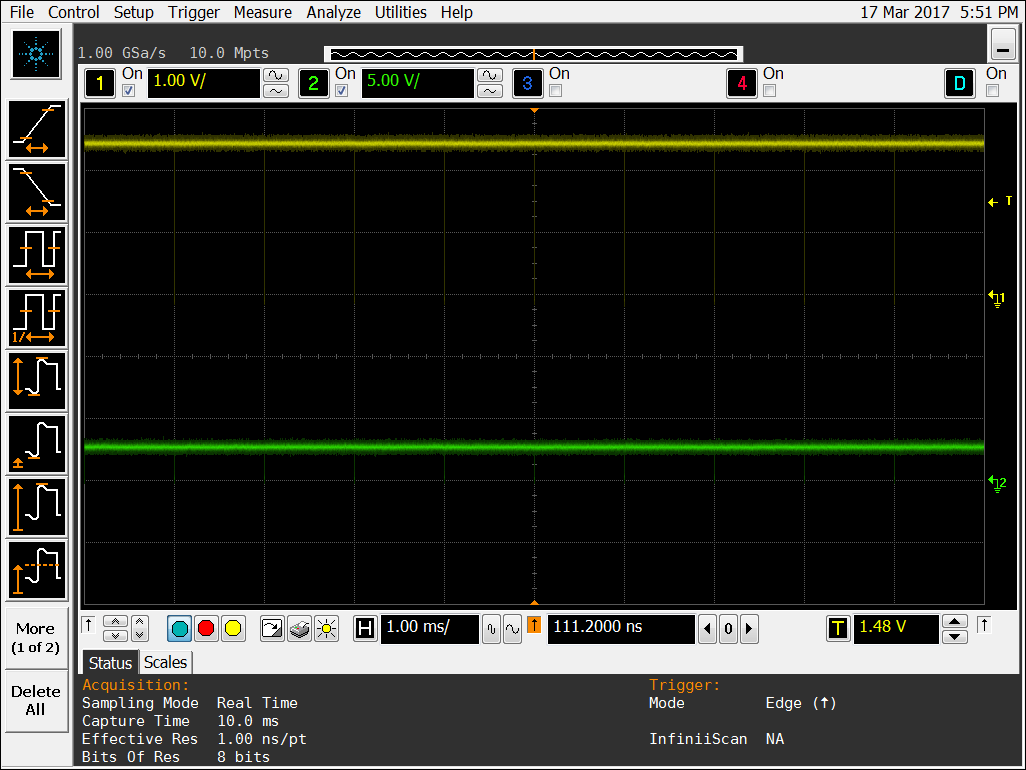
\includegraphics[width=13cm]{1khz_mb_offset_500_ns}
		\caption{1khz signal produced using the internal clock of the rhino}
		\label{fig:1khz_in_500_offset}
	\end{figure}
	
Figure \ref{fig:1khz_in_500_offset} shows the output of the main bang and the digitisation signals measured from the Rhino board. A time division of 1.0 ms was used to display the output.

\subsection{Using an External 100MHz Clock Signal}


\section{Conclusions}

\section{Recommendations}

\end{document}